%compile with pdflatex on papeeria

\documentclass[a4paper,12pt]{article}
\usepackage{fancyhdr}
\usepackage{fancyheadings}
\usepackage[ngerman,german]{babel}
\usepackage{german}
\usepackage[utf8]{inputenc}
%\usepackage[latin1]{inputenc}
\usepackage[active]{srcltx}
%\usepackage{algorithm}
%\usepackage[noend]{algorithmic}
\usepackage{amsmath}
\usepackage{amssymb}
\usepackage{amsthm}
\usepackage{bbm}
\usepackage{enumerate}
\usepackage{graphicx}
\usepackage{ifthen}
\usepackage{listings}
\usepackage{enumitem}
%\usepackage{struktex}
\usepackage{hyperref}
\usepackage{tikz}
\usepackage{float}
\usepackage{subcaption}
\captionsetup{compatibility=false}
\captionsetup[subfigure]{labelformat=empty}

\usepackage{pgfplots}
\pgfplotsset{compat=1.15}
\usepackage{mathrsfs}
\usetikzlibrary{arrows}

\definecolor{ccqqqq}{rgb}{0.8,0,0}

\pagenumbering{gobble}

%%%%%%%%%%%%%%%%%%%%%%%%%%%%%%%%%%%%%%%%%%%%%%%%%%%%%%
%%%%%%%%%%%%%% EDIT THIS PART %%%%%%%%%%%%%%%%%%%%%%%%
%%%%%%%%%%%%%%%%%%%%%%%%%%%%%%%%%%%%%%%%%%%%%%%%%%%%%%
\newcommand{\Fach}{1. Klausur aus der Mathematik (A)}
\newcommand{\Name}{}
\newcommand{\datum}{}
\newcommand{\Matrikelnummer}{}
\newcommand{\Semester}{Q12/1}
\newcommand{\Uebungsblatt}{} %  <-- UPDATE ME
%%%%%%%%%%%%%%%%%%%%%%%%%%%%%%%%%%%%%%%%%%%%%%%%%%%%%%
%%%%%%%%%%%%%%%%%%%%%%%%%%%%%%%%%%%%%%%%%%%%%%%%%%%%%%

\setlength{\parindent}{0em}
\topmargin -1.0cm
\oddsidemargin 0cm
\evensidemargin 0cm
\setlength{\textheight}{9.2in}
\setlength{\textwidth}{6.0in}

%%%%%%%%%%%%%%%
%% Aufgaben-COMMAND
\newcommand{\Aufgabe}[1]{
  {
  \vspace*{0.5cm}
  \textsf{\textbf{Aufgabe #1}}
  \vspace*{0.2cm}
  
  }
}
%%%%%%%%%%%%%%
\hypersetup{
    pdftitle={\Fach{}: Übungsblatt \Uebungsblatt{}},
    pdfauthor={\Name},
    pdfborder={0 0 0}
}

\lstset{ %
language=java,
basicstyle=\footnotesize\tt,
showtabs=false,
tabsize=2,
captionpos=b,
breaklines=true,
extendedchars=true,
showstringspaces=false,
flexiblecolumns=true,
}

\title{Übungsblatt \Uebungsblatt{}}
\author{\Name{}}

\begin{document}
\thispagestyle{fancy}
%\lhead{\sf \large \Fach{} \\ %\small \Name{} - \Matrikelnummer{}
\lhead{\sf \large \Fach{} %\small \Name{} - \Matrikelnummer{}
}
\rhead{\sf \Semester{}   \datum{}}
%\rhead{\sf \Semester{} }
\vspace*{0.2cm}
%\begin{center}
%%\LARGE \sf \textbf{Übungsblatt \Uebungsblatt{}}
%\end{center}
%\vspace*{0.2cm}

%%%%%%%%%%%%%%%%%%%%%%%%%%%%%%%%%%%%%%%%%%%%%%%%%%%%%%
%% Insert your solutions here %%%%%%%%%%%%%%%%%%%%%%%%
%%%%%%%%%%%%%%%%%%%%%%%%%%%%%%%%%%%%%%%%%%%%%%%%%%%%%%

  Name: \underline{\hspace{7cm}}
  \hfill
  Datum: \underline{\hspace{4cm}}

\vspace{0,5cm}Die Rechenwege müssen nachvollziehbar sein!

\vspace{0,5cm} {TEIL A} - ohne Hilfsmittel - Bearbeitungszeit 30 Minuten
\vspace {0,2cm}
 
GEOMETRIE

\Aufgabe{1} 

Gegeben sind die Punkte $A (0|0|0)$ und $ C (5|3|4)$ sowie die Gerade

\[
       g: \vec{X} = \begin{pmatrix}10 \\ -3 \\-4 \end{pmatrix} 
                  + \lambda \begin{pmatrix}5 \\ -3 \\-4 \end{pmatrix}          
\] 
$(\lambda \in \mathbb{R})$

\begin{enumerate}[label={\alph*)}]
\item Zeigen Sie, dass $ g$  eine Mittelsenkrechte von $A$ und $C$ ist.
\item  Die Punkte A und C bilden zusammen mit zwei auf g liegenden Punkten das Quadrat
 $ABCD$. Bestimmen Sie die Koordinaten von B und D.
\end{enumerate}
\begin{flushright}7 BE \end{flushright}


\vspace {0,5cm}
ANALYSIS

\Aufgabe{2:} 
Berechnen Sie die unbestimmten Integrale:

\begin{enumerate}[label={\alph*)}]
  \item $ \int \frac{2x^2}{3x^3-3} dx $
    %\vspace{2,5cm}
  \item $ \int -4xe^{x^2+5} dx $
  %  \vspace{2,5cm}
  %\vspace{1cm}
\end{enumerate}
\begin{flushright}4 BE \end{flushright}
\Aufgabe{3:}
Welche Werte kann $ b \in R\setminus \{ -3\}$ annehmen, damit folgende Gleichung stimmt? Begründen Sie kurz geometrisch und erklären Sie ausführlich!

 $ \int_ {-3}^{b} x^5 dx =0$
\begin{flushright}4 BE \end{flushright}
\begin{flushright}Bitte wenden \end{flushright}
\newpage

\vspace{0,5cm} {TEIL B} -  Hilfsmittel sind zugelassen - Bearbeitungszeit 90 Minuten


\vspace {0,5cm}
ANALYSIS

\Aufgabe{4:}

Finden Sie heraus, welcher der vier Graphen der Graph der Funktion $f(x)$, der Graph der Ableitungsfunktion  $f'(x)$ und der Graph der Stammfunktion  $F(x)$ von f(x)ist. Begründen Sie gründlich unter Verwendung der Fachbegriffen. Ein Graph bleibt übrig.

\begin{figure}[H]
  \centering

    \subfloat[Funktion 1]{
      \begin{tikzpicture}[scale=0.9, line cap=round,line join=round,>=triangle 45,x=1cm,y=1cm]
               \begin{axis}[
           samples=500,domain=-6:5,restrict y to domain =-6:5,
          x=1cm,y=1cm,
          axis lines=middle,
          ymajorgrids=true,
          xmajorgrids=true,
          xmin=-5.3019060283688253,
          xmax=3.9719414893617393,
          ymin=-5.8310602690212177,
          ymax=2.4489042699859294,
          xtick={-5,-4,...,2,3},
          ytick={-5,-4,...,2,3},]
          %\clip(-3.9183806146572397,-3.177277763111059) rectangle (3.1526595744681156,5.299672591498936);
          %\draw[line width=1pt,color=ccqqqq,smooth,samples=100,domain=-2.301906028368825:4.9719414893617384] plot(\x,{e^(\x)-e^(\x)* (\x)^2  )});
            \addplot[line width=1pt,color=ccqqqq ]plot(\x,{e^(\x)-e^(\x)* (\x)^2 -2*e^(\x)* (\x))});
          \begin{scriptsize}
          \draw[color=ccqqqq] (-1.5676861702127871,2.3638422132483394) node {$$};
          \end{scriptsize}
          \end{axis}
        \end{tikzpicture}
    }
    \subfloat[Funktion 2]{

          \begin{tikzpicture}[scale=0.9, line cap=round,line join=round,>=triangle 45,x=1cm,y=1cm]
         %   \begin{axis}[samples=500,domain=-6*pi:6*pi,restrict y to domain =-20:100]

         %\begin{axis}[
         %%samples=500,domain=-5:5,restrict y to domain =-5:5,
         %x=1cm,y=1cm,
         %axis lines=middle,
         %ymajorgrids=true,
         %xmajorgrids=true,
         %    xmin=-5.3019060283688253,
         %    xmax=3.9719414893617393,
         %    ymin=-5.8310602690212177,
         %    ymax=2.4489042699859294,
         %    xtick={-5,-4,...,2,3},
         %    ytick={-5,-4,...,2,3},]
         %   \addplot[line width=1pt,color=ccqqqq ]plot(\x,{e^(\x)-e^(\x)* (\x)^2  )});
         %   \end{axis}

         \begin{axis}[
           samples=500,domain=-6:5,restrict y to domain =-6:5,
          x=1cm,y=1cm,
          axis lines=middle,
          ymajorgrids=true,
          xmajorgrids=true,
          xmin=-5.3019060283688253,
          xmax=3.9719414893617393,
          ymin=-5.8310602690212177,
          ymax=2.4489042699859294,
          xtick={-5,-4,...,2,3},
          ytick={-5,-4,...,2,3},]
          %\clip(-3.9183806146572397,-3.177277763111059) rectangle (3.1526595744681156,5.299672591498936);
          %\draw[line width=1pt,color=ccqqqq,smooth,samples=100,domain=-2.301906028368825:4.9719414893617384] plot(\x,{e^(\x)-e^(\x)* (\x)^2  )});
            \addplot[line width=1pt,color=ccqqqq ]plot(\x,{e^(\x)-e^(\x)* (\x)^2  )});
          \begin{scriptsize}
          \draw[color=ccqqqq] (-1.5676861702127871,2.3638422132483394) node {$$};
          \end{scriptsize}
          \end{axis}
         \end{tikzpicture}


    }      %<------------
\end{figure}


\begin{figure}[H]
  \centering

    \subfloat[Funktion 3]{
      \begin{tikzpicture}[scale=0.9, line cap=round,line join=round,>=triangle 45,x=1cm,y=1cm]
              \begin{axis}[
              x=1cm,y=1cm,
              axis lines=middle,
              ymajorgrids=true,
              xmajorgrids=true,
              xmin=-3.3019060283688253,
              xmax=5.9719414893617393,
              ymin=-2.8310602690212177,
              ymax=5.4489042699859294,
              xtick={-3,-2,...,4,5},
              ytick={-2,-1,...,4,5},]
              %\clip(-3.9183806146572397,-3.177277763111059) rectangle (3.99,5.299672591498936);
        \draw[line width=1pt,color=ccqqqq,smooth,samples=100,domain=-3.6600620567376185:4.488430851063855] plot(\x,{-0.5*(\x)^(4)+1.5*(\x)^3});
              \begin{scriptsize}
              \draw[color=ccqqqq] (-0.69915780141845,-1.5848279995176686) node {$$};
              \end{scriptsize}
              \end{axis}
        \end{tikzpicture}
    }
    \subfloat[Funktion 4]{

          \begin{tikzpicture}[scale=0.9, line cap=round,line join=round,>=triangle 45,x=1cm,y=1cm]
          \begin{axis}[
           samples=500,domain=-6:5,restrict y to domain =-6:5,
          x=1cm,y=1cm,
          axis lines=middle,
          ymajorgrids=true,
          xmajorgrids=true,
          xmin=-5.3019060283688253,
          xmax=3.9719414893617393,
          ymin=-5.8310602690212177,
          ymax=2.4489042699859294,
          xtick={-5,-4,...,2,3},
          ytick={-5,-4,...,2,3},]
          %\clip(-3.9183806146572397,-3.177277763111059) rectangle (3.1526595744681156,5.299672591498936);
          %\draw[line width=1pt,color=ccqqqq,smooth,samples=100,domain=-2.301906028368825:4.9719414893617384] plot(\x,{e^(\x)-e^(\x)* (\x)^2  )});
            \addplot[line width=1pt,color=ccqqqq ]plot(\x,{2+e^(\x)-(e^(\x)* ((\x)^2 -2*(\x)+2)))});
          \begin{scriptsize}
          \draw[color=ccqqqq] (-1.5676861702127871,2.3638422132483394) node {$$};
          \end{scriptsize}
          \end{axis}
          \end{tikzpicture}


    }      %<------------
\end{figure}

\begin{flushright}6 BE \end{flushright}
\newpage





\Aufgabe {5:} 
Der Rand eines Segels (siehe Abbildung) wird näherungsweise von jeweils einem Teil des Graphen $G_f$ der Funktion $f: f(x)=x+6-\frac{32}{x^2}$;
$ \mathbb{D}_f= \mathbb{R}\setminus \{0\}$, der x-Achse und der Geraden g mit der Gleichung: $g(x)=x+4$ gebildet.

\begin{figure}[h!]
  \begin{center}
    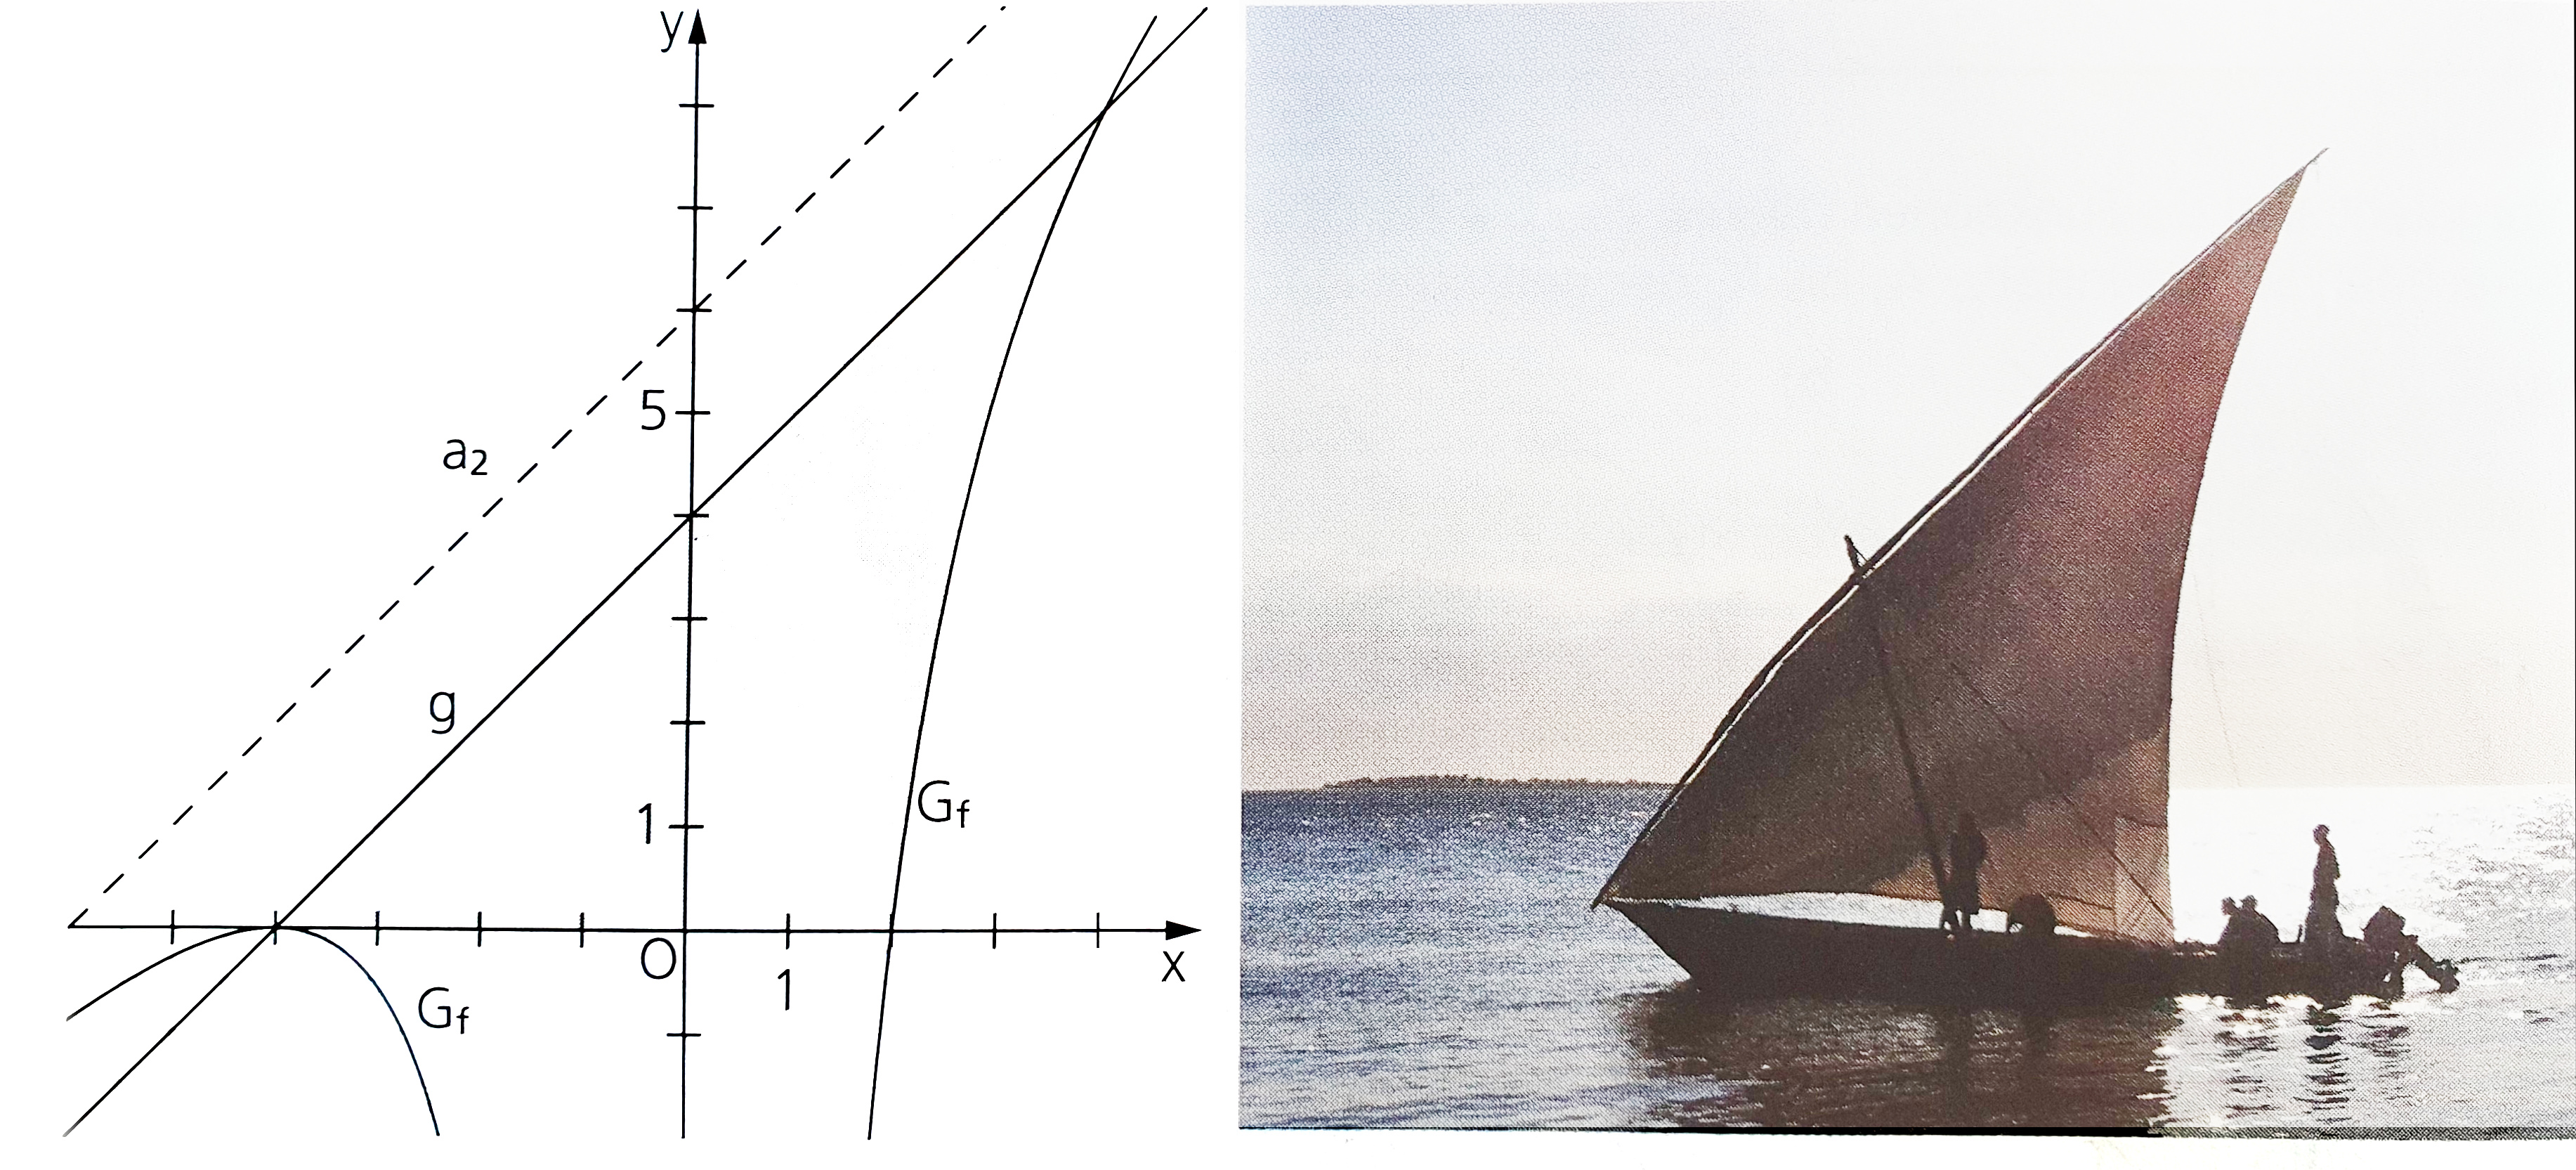
\includegraphics[width=1 \linewidth]{bols201202.jpeg}
    %\caption{A boat.}
    %\label{fig:boat1}
  \end{center}
\end{figure}

\begin{enumerate}[label={\alph*)}]
\item Berechnen Sie den Flächeninhalt des Segels (1LE=1m).
\item Um maximal die Windstärke zu nutzen, soll die obere Kante des Segels den Hochpunkt der Funktion f(x) mit dem Schnittpunkt der Funktionen f(x) und g(x) verbinden. Begründen Sie rechnerisch, dass das Segel hier diese Bedingung erfüllt. 
\end{enumerate}  
\begin{flushright}8 BE \end{flushright}
\begin{flushright}Bitte wenden \end{flushright}
\newpage
\addtolength{\voffset}{-2cm}

GEOMETRIE
\Aufgabe{6:} 
Die folgende Abbildung zeigt modellhaft eine Tribüne, die auf einer horizontalen Fläche steht.

\begin{figure}[h!]
  \begin{center}
    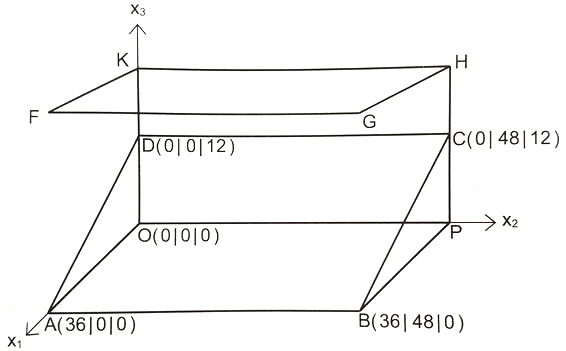
\includegraphics[width=0.5\linewidth]{tribüne.jpg}
    %\caption{A boat.}
    %\label{fig:boat1}
  \end{center}
\end{figure}


\enlargethispage{2cm}

Dabei beschreibt das Rechteck ABCD mit
  $A (36|0|0)$, $ B (36|48|0)$, $C (0|48|12)$ und $ D (0|0|12) $
die Nutzfläche der Tribüne. Das Rechteck ABPO stellt die Grundfläche der Tribüne dar, das
Rechteck FGHK beschreibt die Dachfläche der Tribüne. Die Eckpunkte der Dachfläche liegen
senkrecht über den entsprechenden Eckpunkten der Grundfläche.
Die $x_1x_2 $  Ebene stellt den Erdboden dar. Die $ x_1$ – Achse zeigt nach Süden, die $x_2$ – Achse nach
Osten. Eine Längeneinheit im Koordinatensystem entspricht 1m in der Realität, d.h. die Tribüne ist
48m breit. Die Materialstärke ist bei den Rechnungen zu vernachlässigen.
\begin{enumerate}[label={\alph*)}]
\item  Bestimmen Sie eine Gleichung der Ebene N, in der das Rechteck ABCD liegt, in
Normalenform. (zur Kontrolle:$ x_1 + 3x_3 = 36 $)
\item Berechnen Sie die Größe des Neigungswinkels der Nutzfläche gegen die Horizontale.
\item Die Dachfläche liegt im Modell in der Ebene $E: x_1 - 6x_3 + 96 = 0.$
Ermitteln Sie die Koordinaten des Punktes G, der im Modell einen Dachflächeneckpunkt
darstellt und senkrecht über dem Punkt B liegt. (zur Kontrolle: $G (36|48|22)$)
\item Zur Installation von Lautsprechern soll eine Metallstange so an der Tribüne befestigt
werden, dass sie an dem Punkt beginnt, der im Modell durch den Punkt $G (36|48|22)$  beschrieben wird
und an der Nutzflächenkante endet, die im Modell durch die Strecke [BC] dargestellt wird.
Aus Kostengründen soll die Stange so kurz wie möglich sein. Untersuchen Sie, ob eine 20m
lange Stange ausreicht.
\item An der Dachflächenkante Richtung Spielstätte, im Modell dargestellt durch die Strecke
[FG], soll eine Regenrinne abgehängt werden. Ein Befestigungspunkt R liegt 2 cm
unterhalb von G. Die Lage des zweiten Befestigungspunktes wird unterhalb von F so
gewählt, dass die Regenrinne auf einer horizontalen Länge von 2 m um 2 mm abfällt. Das
Wasser soll dabei Richtung Westen abfließen. Geben Sie eine Gleichung der Geraden h an,
die den Verlauf der Regenrinne zwischen den Befestigungspunkten im Modell beschreibt.
\end{enumerate}
%\vspace{-0,7cm}


\begin{flushright}18 BE \end{flushright}
%\enlargethispage{2\baselineskip}

%\addtolength{\voffset}{-2cm}




%\begin{tikzpicture}
%\draw [very thin, black, step=0.5cm] (0,0) grid +(15,18);
%\end{tikzpicture}




%%%%%%%%%%%%%%%%%%%%%%%%%%%%%%%%%%%%%%%%%%%%%%%%%%%%%%
%%%%%%%%%%%%%%%%%%%%%%%%%%%%%%%%%%%%%%%%%%%%%%%%%%%%%%
\end{document}
